\documentclass{report}
%Configuration page
\usepackage{geometry}
\geometry{
	width=21.59cm, 
	height=27.94cm,
	left=3.17cm,
	right=3.81cm,
	bottom=3.81cm,
	top=3.17cm,
}

%...............................................................
%Tamaño para titulos de chapters,secciones,subsecciones
\usepackage{sectsty}
\usepackage{titlesec}
\sectionfont{\large}
\subsectionfont{\large}
%...............................................................
%figures and Tables 
\usepackage{caption}
\usepackage{subcaption}
%...............................................................
%Using Packages (general)
\usepackage[utf8]{inputenc}
\usepackage[T1]{fontenc, url}
\usepackage[spanish,es-tabla]{babel}
\usepackage{times} %Use Font Times New Roman 
\usepackage{amsmath}
\usepackage{amsfonts}
\usepackage{amssymb}
\usepackage{makeidx}
\usepackage{graphicx}
\graphicspath{{figures/}} %Import images from folder
\usepackage{float}
\usepackage[table,xcdraw]{xcolor}
\usepackage[toc,page]{appendix}
%...............................................................
%Comments
\usepackage{comment}%Comments in file  
\usepackage[colorinlistoftodos]{todonotes}%Comments in pdf
%...............................................................
%Generic text packages 
\usepackage{blindtext}
\usepackage{lipsum}
%...............................................................
%Change tables, contents, figures parameters 
\usepackage{tocloft}
\usepackage{tocenter}
\usepackage{gensymb} %Degree Symbol
\usepackage{textcomp} %Symbols 
\usepackage{chngpage}% allows for temporary adjustment of side margins
%...............................................................
%Page style
\usepackage{fancyhdr}
\pagestyle{fancy}
\fancyhf{}
\lhead{Pontificia Universidad Javeriana}
\rhead{Memoria de Trabajo de Grado - Profundización}
\rfoot{Página \thepage}
\renewcommand{\headrulewidth}{0.5pt}
\renewcommand{\footrulewidth}{0.5pt}
%...............................................................
%Redefine plain (chapters, tables, appendix)
\fancypagestyle{plain}{
\fancyhf{}
\fancyhead[OL]{Pontificia Universidad Javeriana}
\fancyhead[OR]{Memoria de Trabajo de Grado - Profundización}
\fancyfoot[R]{Página \thepage}
\fancyfoot[L]
}
%...............................................................
% To make cites and references
\usepackage[hidelinks,pdfusetitle,pdfdisplaydoctitle]{hyperref} 
\usepackage{doi}
\renewcommand{\doitext}{}
\usepackage{natbib} %Package to cite references
%...............................................................
% To make pretty tables
\usepackage{booktabs}
\usepackage{multirow}
\usepackage{dcolumn}
\usepackage{array}
%Control de terminaciones de linea en párrafo
\hyphenpenalty=100000   % No se dividen las palabras al terminar una línea
\sloppy % Ayuda a que las cosas no se salgan de los márgenes.
\raggedbottom % Hace que el tamaño de las páginas llegue hasta donde llegue el texto, no agrega espacio vertical

%----------------------------------------------------------------------------%
\begin{document}

    \thispagestyle{empty}
\newcommand{\CODIGOTG}{12345}
\newcommand{\TITULOTG}{ Evaluación e implementación de métodos de extracción automática de palabras clave aplicados a textos cortos en español}
\newcommand{\AUTORESTG}{Kelly Gisselle Candelo\\
Andrea Guti{\'e}rrez Ladino\\
Iv{\'a}n Felipe Molano}
\newcommand{\DIRECTORTG}{Alexandra Pomares Quimbaya}

\begin{center}
	%\vspace{0.1cm}
		\vspace*{2cm}
		\fontsize{16pt}{16pt}\textbf{\CODIGOTG\ }\\
		\fontsize{14pt}{14pt}\selectfont \TITULOTG\ \\ %Modificar de acuerdo a la facultad
%............................................................................	
		\vspace*{5cm}
		\fontsize{14pt}{14pt}\selectfont Autores\\
		\AUTORESTG\ \\
		%Debajo del título con 
%............................................................................
		\vspace*{5cm}
		\fontsize{14pt}{14pt}\selectfont PONTIFICIA UNIVERSIDAD JAVERIANA\\
		FACULTAD DE INGENIERIA\\
		MAESTRÍA EN INGENIERÍA DE DE SISTEMAS Y COMPUTACIÓN\\
		BOGOTÁ, D.C.\\
		2021 
\end{center}


    \thispagestyle{empty}

\begin{center}

		\fontsize{12pt}{12pt}\textbf{<CÓDIGO>}\\
		\fontsize{14pt}{14pt}\selectfont Título del Trabajo de Grado\\ %Modificar de acuerdo a la facultad
%............................................................................	
		\vspace*{3cm}
		\fontsize{12pt}{12pt}\textbf{Autor:}\\ 
		\vspace{0.2cm}
		\fontsize{14pt}{14pt}Nombre Completo del Autor\\
%............................................................................
        \vspace*{4cm}
		\fontsize{12pt}{12pt}{MEMORIA DEL TRABAJO DE GRADO REALIZADO PARA CUMPLIR UNO DE LOS REQUISITOS PARA OPTAR AL TITULO DE MAGÍSTER EN INGENIERÍA DE SISTEMAS Y COMPUTACIÓN}

%............................................................................
        \vspace*{1.7cm}
		\fontsize{12pt}{12pt}\textbf{Directora}\\
		\vspace{0.2cm}
        Nombre completo del director del TG\\
        \vspace{0.2cm}
        \textbf{Comité de Evaluación del Trabajo de Grado}\\
        \vspace{0.2cm}
        <Nombres y Apellidos Completos del Jurado >\\
        \vspace{0.2cm}
        <Nombres y Apellidos Completos del Jurado >\\
        \vspace{0.2cm}
        \textbf{Página web del Trabajo de Grado}\\
        \vspace{0.2cm}
        http://pegasus.javeriana.edu.co/~<código>\\
%............................................................................

		\vspace*{1.8cm}
		\fontsize{12pt}{12pt}\selectfont PONTIFICIA UNIVERSIDAD JAVERIANA\\
		FACULTAD DE INGENIERIA\\
		MAESTRÍA EN INGENIERÍA DE DE SISTEMAS Y COMPUTACIÓN\\
		BOGOTÁ, D.C.\\
		<MES><AÑO> %Modificar de acuerdo al año vigente
\end{center}
    \thispagestyle{empty}

\begin{center}

		\fontsize{12pt}{12pt}\textbf{PONTIFICIA UNIVERSIDAD JAVERIANA\\
		FACULTAD DE INGENIERIA\\
		MAESTRÍA EN INGENIERÍA DE SISTEMAS Y COMPUTACIÓN}\\
%............................................................................	
        \vspace*{10cm}
		\fontsize{12pt}{12pt}\selectfont \textbf{Rector Magnífico}\\
		\vspace{0.2cm}
        Jorge Humberto Peláez, S.J.\\
        \vspace{0.2cm}
        \textbf{Decano Facultad de Ingeniería}\\
        \vspace{0.2cm}
        Ingeniero Lope Hugo Barrero Solano\\
        \vspace{0.2cm}
        \textbf{Director Maestría en Ingeniería de Sistemas y Computación}\\
        \vspace{0.2cm}
        Ingeniera Angela Carrillo Ramos\\
        \vspace{0.2cm}
        \textbf{Director Departamento de Ingeniería de Sistemas}\\
        \vspace{0.2cm}
        Ingeniero Efraín Ortíz Pabón\\
        
\end{center}
    \setcounter{page}{4}
%..................................	
	%Sections 
	\begin{flushleft}
		\phantomsection \label{artículo}
		\vspace*{2cm}
		\large{\textbf{Artículo 23 de la Resolución No. 1 de Junio de 1946}}
	\end{flushleft}
	\input{Resolución}
	\clearpage

%..................................	
	%Sections 
	\begin{center}
		\phantomsection \label{glads}
		\large{\textbf{AGRADECIMIENTOS}}
	\end{center}
	\fontsize{11pt}{11pt}\selectfont %Cambiar si se desea letra más grande
\vspace*{0.2cm}
Escribir un mensaje en caso de que sienta agradecimiento por alguien que lo haya apoyado en el desarrollo del Trabajo de Grado. Su fami-lia, su pareja, sus amigos, su director, sus profesores, etc\\
	\clearpage
%..................................	
    %\fontsize{11pt}{11pt}\selectfont %Cambiar si se desea letra más grande 
\vspace*{0.2cm}
\begin{center}
    \fontsize{14pt}{14pt}\textbf{ABSTRACT}\\
\end{center}
\vspace*{0.2cm}
\noindent Write a paragraph in English in which a reader could understand what the problem was and what you have done to resolve it. Maximum 100 words.  You can support this activity by reading the information that you can find in the following hyperlinks:
%-----------------------------------------------------------------------------
\vspace*{1.5cm}
\begin{center}
    \fontsize{14pt}{14pt}\textbf{RESUMEN}\\
\end{center}
\vspace*{0.2cm}
\noindent Escriba un párrafo en el cual un lector pueda entender cuál fue el problema y qué se hizo para resolverlo. Máximo 100 palabras. Usted puede utilizar la información contenida en los siguientes enlaces para escribir un buen abstract o resumen:

%..................................	
    \begin{center}
		\phantomsection \label{resumenejecutivo}
		\large{\textbf{RESUMEN EJECUTIVO}}
	\end{center}
	\fontsize{11pt}{11pt}\selectfont %Cambiar si se desea letra más grande 
\vspace*{0.5cm}
Describa brevemente la problemática, diga lo que se hizo y presente los resultados y conclu-siones principales que se obtuvieron con su realización. Mínimo 1000 palabras, máximo 1200.
	\clearpage

%..................................	
    \setlength{\cftbeforetoctitleskip}{-0.3cm}
	\renewcommand{\cfttoctitlefont}{\large}
	\renewcommand{\contentsname}{\textbf{CONTENIDO}}
	
	\tableofcontents 
	\newpage
	\renewcommand\cftloftitlefont{\large}
	\renewcommand{\listfigurename}{\textbf{ÍNDICE DE FIGURAS}}
	%\listoffigures
	{%
		\let\oldnumberline\numberline%
		\renewcommand{\numberline}{\figurename~\oldnumberline}%
		\listoffigures%
	}
	\newpage
	\renewcommand\cftlottitlefont{\large}
	\renewcommand{\listtablename}{\textbf{ÍNDICE DE TABLAS}}
	{%
		\let\oldnumberline\numberline%
		\renewcommand{\numberline}{\tablename~\oldnumberline}%
		\listoftables%
	}
	\newpage
%..................................	
	%\pagenumbering{arabic} % Comienza la numeración arábiga (números normales)
	%\setcounter{page}{1} % Comienza el contador de páginas en 1
%..................................	
	\chapternumberfont{\huge}
	\chaptertitlefont{\large}
	\chapter{INTRODUCCIÓN}
	\input{chapters/Introducción}
	
	\chapter*{Foreword} 
    \addcontentsline{toc}{chapter}{Foreword}
%..................................	
	\chapter{DESCRIPCIÓN GENERAL}
	\fontsize{14}{15}\selectfont

\section{OPORTUNIDAD Y PROBLEMÁTICA}
\blindtext\\


%..................................	
	\chapter{DESCRIPCIÓN DEL PROYECTO}
	\fontsize{14}{15}\selectfont
\setcounter{secnumdepth}{5}

\section{OBJETIVO GENERAL}
Evaluar la adaptación de las técnicas existentes de extracción de palabras clave en el contexto de textos cortos formales y semi-informales en español.

\section{OBJETIVOS ESPECÍFICOS}
\begin{itemize}
  \item Caracterizar el conjunto de técnicas de extracción de palabras clave más representativas o adaptables al idioma español.
  \item Implementar una adaptación de los 3 métodos más relevantes arrojados en el análisis de técnicas encontradas.
  \item Evaluar la aplicación de los métodos para determinar cuáles son sus características de desempeño, frente a textos cortos formales y semi-informales en español, en el dominio específico de los registros de llamadas de usuarios del servicio de Mentes Colectivas de la Pontificia Universidad Javeriana.
\end{itemize}


\section{FASES DE DESARROLLO}
Para el desarrollo del Proyecto en general, se aplicará la metodología Scrum, planteando Spritns de dos semanas, durante las cuales se establecerán diferentes tareas. \par
Para lo que corresponde a la aplicación específica sobre los registros de llamadas de los usuarios del servicio de Mentes Colectivas, se aplicará la metodología CRISP-DM (Cross-Industry Standard Process for Data Mining). 

\subsection{Metodología CRISP-DM}
La metodología CRISP-DM es una de las metodologías más utilizadas en proyectos de minería de datos; dicha metodología es representada como un ciclo, en el cual se ejecu-tan 6 fases que no necesariamente son dependientes la una de la otra, ya que se permite (en algunas fases) realizar retornos a fases anteriores, permitiendo así, generar mejores resultados sobre el proyecto. A continuación, se presenta una ilustración del ciclo de minería de datos según CRISP-DM:

\begin{figure}[h]
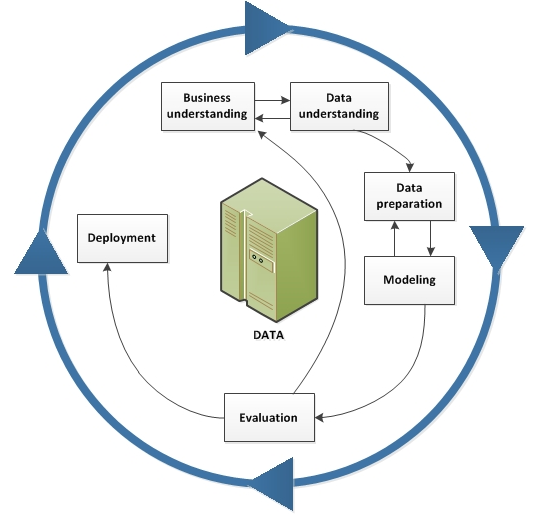
\includegraphics[scale=0.7]{Documento Trabajo de Grado/figures/CicloDeVidaCRISPDM.png}
\centering
\caption{Ciclo de Vida CRISP-DM}
\centering
\end{figure}

La metodología CRISP-DM está compuesta por las fases enumeradas en las siguientes secciones.

\subsubsection{Entendimiento del Negocio}
Esta primera fase busca 
\subsubsection{Entendimiento de los Datos}
\subsubsection{Preparación de los Datos}
\subsubsection{Modelamiento}
\subsubsection{Evaluación}
\subsubsection{Despliegue}


\subsection{Metodología SCRUM}
%..................................	
	\chapter{MARCO TEÓRICO / ESTADO DEL ARTE}
	\fontsize{14}{15}\selectfont

\section{MINERÍA DE DATOS}
\blindtext\\


\section{METODOLOGÍA CRISP-DM}
\blindtext\\
\subsection{Entendimiento del Negocio}
\blindtext\\
\subsection{Entendimiento de los datos}
\blindtext\\
\subsection{Preparación de los datos}
\blindtext\\
\subsection{Modelamiento}
\blindtext\\
\subsection{Evaluación}
\blindtext\\


\section{ENFOQUES DE EXTRACCIÓN DE PALABRAS CLAVE}
\blindtext\\
\subsection{Basados en reglas de lenguajes}
\blindtext\\
\subsection{Estadísticos}
\blindtext\\
\subsection{Basados en grafos}
\blindtext\\
\subsection{Machine Learning}
\blindtext\\


\section{TIPOS DE TEXTOS}
\blindtext\\
\subsection{Formales}
\blindtext\\
\subsection{Semi-informales}
\blindtext\\
\subsection{Informales}
\blindtext\\

%..................................	
	\chapter{TRABAJOS RELACIONADOS}
	


%..................................	
	\chapter{DESARROLLO DEL PROYECTO}
	\fontsize{14}{15}\selectfont

\section{Entendimiento del negocio}
\blindtext\\
\subsection{Objetivos de negocio}
\blindtext\\
\subsection{Evaluación de la situación}
\blindtext\\
\subsection{Objetivos de minería de datos}
\blindtext\\
\subsection{Plan de proyecto}
\blindtext\\

%--------------------------------------------------------------------
\section{Recolección de datos}
\blindtext
\subsection{Descripción de los datos}
\blindtext\\
\subsection{Exploración de los datos}
\blindtext\\
\subsection{Calidad de los datos}
\blindtext\\

%--------------------------------------------------------------------

\section{Preparación de los Datos}
\blindtext
\subsection{Selección de datos}
\blindtext\\
\subsection{Limpieza de datos}
\blindtext\\
\subsection{Construcción de datos}
\blindtext\\
\subsection{Integración de datos}
\blindtext\\
\subsection{Formato de datos}
\blindtext\\
\subsection{Descripción del set de datos final}
\blindtext\\

%--------------------------------------------------------------------
\section{Modelamiento}
\blindtext
\subsection{Selección de técnicas de modelamiento}
\blindtext\\
\subsection{Diseño plan de prueba}
\blindtext\\
\subsection{Construcción del modelo}
\blindtext\\

%--------------------------------------------------------------------

\section{Evaluación}
\blindtext
\subsection{Evaluación de resultados}
\blindtext\\
\subsection{Pasos a seguir}
\blindtext\\
	\clearpage
%..................................	
	\addcontentsline{toc}{chapter}{REFERENCIAS}
	\renewcommand{\bibname}{REFERENCIAS}
	\bibliographystyle{apalike}
	\setstretch{1}
	\setlength{\bibsep}{2em plus 0.5ex}
	\bibliography{references/papers} %Link a referencias
	\clearpage
%..................................	
	\appendix
	\renewcommand{\appendixname}{ANEXOS}
	\renewcommand{\appendixpagename}{ANEXOS}
	\renewcommand{\appendixtocname}{ANEXOS}
	\addappheadtotoc	
	\fontsize{12pt}{14.5}\selectfont
\chapter{Tablas y gráficos de conexión} \label{anexo1}
\section{Tablas Series de Tiempo}
%............Table:style2.........................%
\begin{table}[ht]
	\centering
	\setlength{\arrayrulewidth}{1mm}
	\renewcommand{\arraystretch}{2.5}
	\arrayrulecolor{white}
	\begin{tabular}{|l|l|l|l|l|l|}
		\hline
		\rowcolor[HTML]{E0E0E0} 
		{\color[HTML]{000000} \textbf{Ciudad}} & {\color[HTML]{000000} \textbf{Número}} & {\color[HTML]{000000} \textbf{Edificio 1}} & {\color[HTML]{000000} \textbf{Remodelación 1}} & {\color[HTML]{000000} \textbf{Valor[millones]}} & {\color[HTML]{000000} \textbf{Tiempo}} \\ \hline
		\rowcolor[HTML]{EFEFEF} 
		{\color[HTML]{000000} París}               & {\color[HTML]{000000} 361}           & {\color[HTML]{000000} 11 Ago 2007}         & {\color[HTML]{000000} 24 Nov 2007}         & {\color[HTML]{000000} $\sim$135}            & {\color[HTML]{000000} 105 días}            \\ \hline
		\rowcolor[HTML]{EFEFEF} 
		{\color[HTML]{000000} New York}              & {\color[HTML]{000000} 368}           & {\color[HTML]{000000} 10 Oct 2007}         & {\color[HTML]{000000} 24 Nov 2007}         & {\color[HTML]{000000} $\sim$259}            & {\color[HTML]{000000} 35 días}             \\ \hline
		\rowcolor[HTML]{EFEFEF} 
		{\color[HTML]{000000} Zurich}              & {\color[HTML]{000000} 96}            & {\color[HTML]{000000} 05 Nov 2007}         & {\color[HTML]{000000} 10 Dic 2007}         & {\color[HTML]{000000} $\sim$-204 }            & {\color[HTML]{000000} 35 días}             \\ \hline
	\end{tabular}
	\label{table:1anexo1}
\end{table}
%............................................%
\newpage %Cambiar de página
\section{Gráficos de Conexión}
\chapter{Lugares extras} \label{anexo2}
\section{Lugar extra 1}
\begin{figure}[h]
	\centering
	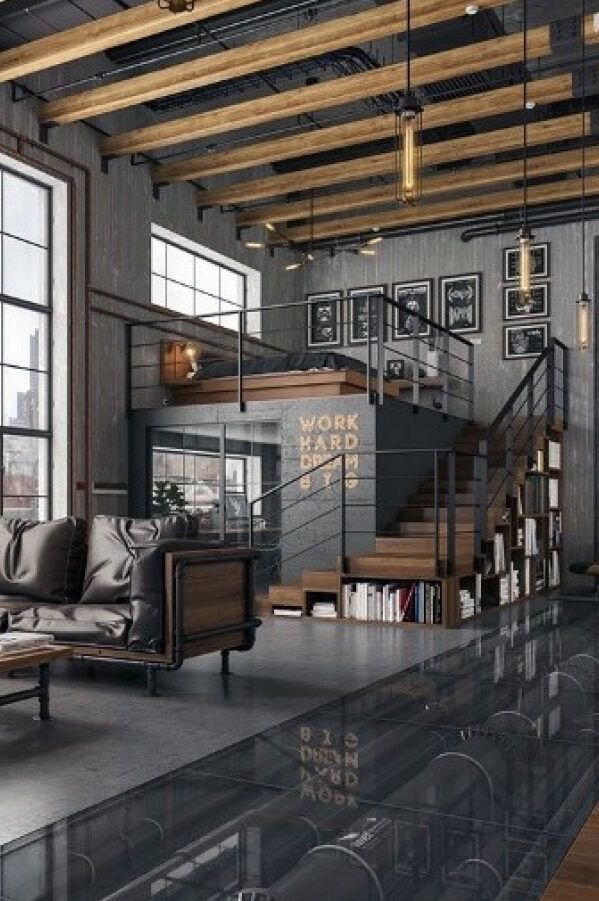
\includegraphics[scale=0.4]{figure4} 
	\label{ilustracion4} 
\end{figure}

\end{document}
